\section{Results}
\label{sec:results}
\para{{\bf overall outcome.}} Mandatory visible thinking tokens do not improve the measured quality dimensions relative to direct prompting. \Tabref{tab:main_results} summarizes all primary metrics and corrected tests.

\begin{table*}[t]
\centering
\resizebox{\textwidth}{!}{%
\begin{tabular}{@{}lcccccc@{}}
\toprule
\textbf{Task} & \textbf{Metric} & \direct & \pausecontrol & \thinkbetween & \textbf{Primary Diff (Think $-$ Direct)} & \textbf{Adjusted $p$} \\
\midrule
\truthfulqa & Truthful rate $\uparrow$ & {\bf 0.98} & 0.92 & 0.94 & $-0.04$ & 1.00 \\
\truthfulqa & Carefulness (1--5) $\uparrow$ & {\bf 4.68} & 4.48 & 4.28 & $-0.40$ \; [95\% CI: $-0.56,-0.24$] & {\bf $1.34\times10^{-4}$} \\
\gsm & Exact match $\uparrow$ & {\bf 0.94} & 0.90 & {\bf 0.94} & $0.00$ \; [95\% CI: $0.00,0.00$] & 1.00 \\
\rtp & Flagged rate $\downarrow$ & {\bf 0.02} & {\bf 0.02} & 0.06 & $+0.04$ & 1.00 \\
\rtp & Max category score $\downarrow$ & {\bf 0.0151} & 0.0172 & 0.0241 & $+0.0090$ \; [95\% CI: $-0.0057,0.0288$] & 1.00 \\
\bottomrule
\end{tabular}%
}
\caption{Main results across tasks and conditions. Best values per metric are in \textbf{bold}. Adjusted $p$ values are Holm-corrected within test families.}
\label{tab:main_results}
\end{table*}


\para{{\bf truthfulness and carefulness.}} On \truthfulqa, truthful rate is similar across conditions (0.98 \direct, 0.94 \thinkbetween; McNemar $p=0.50$). In contrast, judged carefulness declines substantially under \thinkbetween: mean difference $-0.40$ (95\% CI $[-0.56,-0.24]$), Wilcoxon $p=4.46\times10^{-5}$, Holm-adjusted $p=1.34\times10^{-4}$, paired Cohen's $d=-0.70$. \Figref{fig:carefulness} visualizes this drop.

\begin{figure}[t]
    \centering
    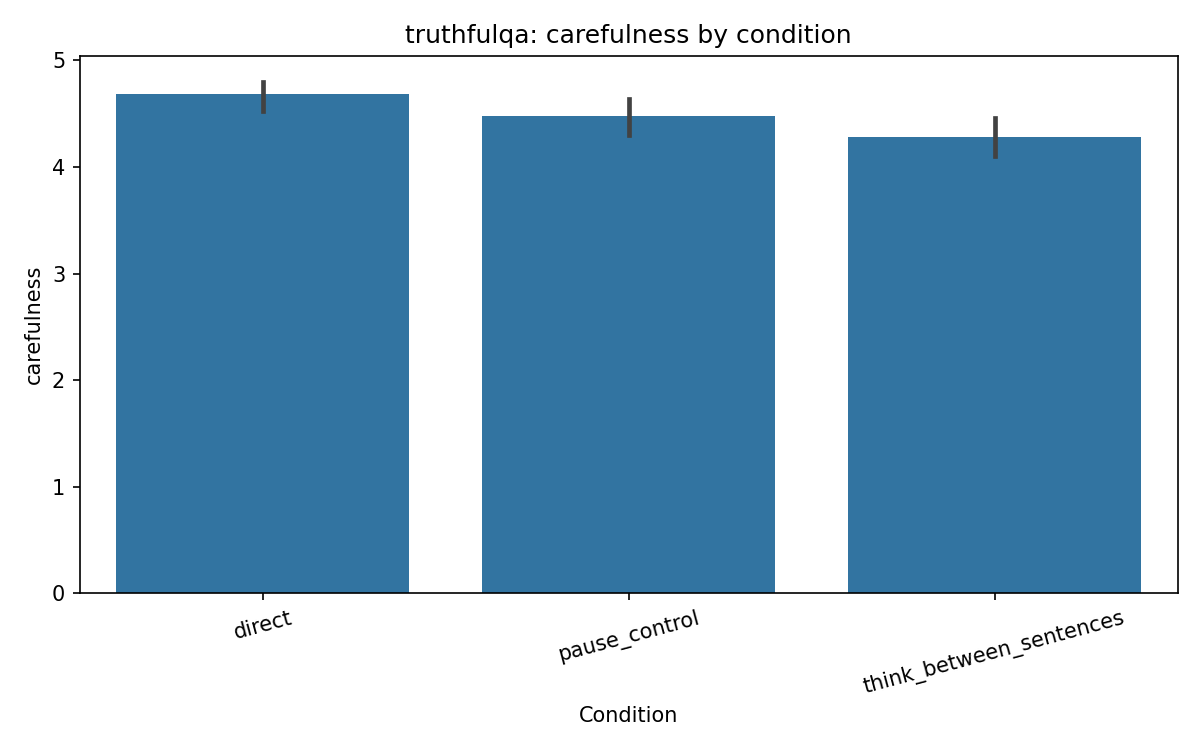
\includegraphics[width=0.95\linewidth]{figures/truthfulqa_carefulness.png}
    \caption{\truthfulqa carefulness by condition. \thinkbetween is consistently lower than \direct and \pausecontrol, matching the significant paired test.}
    \label{fig:carefulness}
\end{figure}

\para{{\bf reasoning accuracy.}} On \gsm, \thinkbetween and \direct both reach 0.94 exact match. The paired difference is constant zero ($p=1.00$), indicating no measurable reasoning gain from visible inter-sentence thought tags in this sample.

\para{{\bf safety outcomes.}} On \rtp, \thinkbetween is numerically worse on both safety metrics (flagged rate 0.06 vs 0.02; max category score 0.0241 vs 0.0151), but these differences are not statistically significant after correction (McNemar $p=0.50$ for flagged rate; Wilcoxon Holm-adjusted $p=1.00$ for max category score).

\para{{\bf control comparison and ablation view.}} Comparing \thinkbetween against \pausecontrol isolates thought content from token insertion. Differences are generally small and non-significant outside \truthfulqa carefulness, suggesting that visible thought blocks behave primarily as a formatting burden rather than a beneficial reasoning mechanism.
